
%% bare_conf.tex
%% V1.3
%% 2007/01/11
%% by Michael Shell
%% See:
%% http://www.michaelshell.org/
%% for current contact information.
%%
%% This is a skeleton file demonstrating the use of IEEEtran.cls
%% (requires IEEEtran.cls version 1.7 or later) with an IEEE conference paper.
%%
%% Support sites:
%% http://www.michaelshell.org/tex/ieeetran/
%% http://www.ctan.org/tex-archive/macros/latex/contrib/IEEEtran/
%% and
%% http://www.ieee.org/

%%*************************************************************************
%% Legal Notice:
%% This code is offered as-is without any warranty either expressed or
%% implied; without even the implied warranty of MERCHANTABILITY or
%% FITNESS FOR A PARTICULAR PURPOSE! 
%% User assumes all risk.
%% In no event shall IEEE or any contributor to this code be liable for
%% any damages or losses, including, but not limited to, incidental,
%% consequential, or any other damages, resulting from the use or misuse
%% of any information contained here.
%%
%% All comments are the opinions of their respective authors and are not
%% necessarily endorsed by the IEEE.
%%
%% This work is distributed under the LaTeX Project Public License (LPPL)
%% ( http://www.latex-project.org/ ) version 1.3, and may be freely used,
%% distributed and modified. A copy of the LPPL, version 1.3, is included
%% in the base LaTeX documentation of all distributions of LaTeX released
%% 2003/12/01 or later.
%% Retain all contribution notices and credits.
%% ** Modified files should be clearly indicated as such, including  **
%% ** renaming them and changing author support contact information. **
%%
%% File list of work: IEEEtran.cls, IEEEtran_HOWTO.pdf, bare_adv.tex,
%%                    bare_conf.tex, bare_jrnl.tex, bare_jrnl_compsoc.tex
%%*************************************************************************

% *** Authors should verify (and, if needed, correct) their LaTeX system  ***
% *** with the testflow diagnostic prior to trusting their LaTeX platform ***
% *** with production work. IEEE's font choices can trigger bugs that do  ***
% *** not appear when using other class files.                            ***
% The testflow support page is at:
% http://www.michaelshell.org/tex/testflow/



% Note that the a4paper option is mainly intended so that authors in
% countries using A4 can easily print to A4 and see how their papers will
% look in print - the typesetting of the document will not typically be
% affected with changes in paper size (but the bottom and side margins will).
% Use the testflow package mentioned above to verify correct handling of
% both paper sizes by the user's LaTeX system.
%
% Also note that the "draftcls" or "draftclsnofoot", not "draft", option
% should be used if it is desired that the figures are to be displayed in
% draft mode.
%
\documentclass[10pt, conference, compsocconf]{IEEEtran}
% Add the compsoc option for Computer Society conferences.
%
% If IEEEtran.cls has not been installed into the LaTeX system files,
% manually specify the path to it like:
% \documentclass[conference]{../sty/IEEEtran}
% Some very useful LaTeX packages include:
% (uncomment the ones you want to load)


% *** MISC UTILITY PACKAGES ***
%
%\usepackage{ifpdf}
% Heiko Oberdiek's ifpdf.sty is very useful if you need conditional
% compilation based on whether the output is pdf or dvi.
% usage:
% \ifpdf
%   % pdf code
% \else
%   % dvi code
% \fi
% The latest version of ifpdf.sty can be obtained from:
% http://www.ctan.org/tex-archive/macros/latex/contrib/oberdiek/
% Also, note that IEEEtran.cls V1.7 and later provides a builtin
% \ifCLASSINFOpdf conditional that works the same way.
% When switching from latex to pdflatex and vice-versa, the compiler may
% have to be run twice to clear warning/error messages.






% *** CITATION PACKAGES ***
%
%\usepackage{cite}
% cite.sty was written by Donald Arseneau
% V1.6 and later of IEEEtran pre-defines the format of the cite.sty package
% \cite{} output to follow that of IEEE. Loading the cite package will
% result in citation numbers being automatically sorted and properly
% "compressed/ranged". e.g., [1], [9], [2], [7], [5], [6] without using
% cite.sty will become [1], [2], [5]--[7], [9] using cite.sty. cite.sty's
% \cite will automatically add leading space, if needed. Use cite.sty's
% noadjust option (cite.sty V3.8 and later) if you want to turn this off.
% cite.sty is already installed on most LaTeX systems. Be sure and use
% version 4.0 (2003-05-27) and later if using hyperref.sty. cite.sty does
% not currently provide for hyperlinked citations.
% The latest version can be obtained at:
% http://www.ctan.org/tex-archive/macros/latex/contrib/cite/
% The documentation is contained in the cite.sty file itself.


\usepackage{graphicx}



% *** GRAPHICS RELATED PACKAGES ***
%
\ifCLASSINFOpdf
  %\usepackage[pdftex]{graphicx}
  % declare the path(s) where your graphic files are
  % \graphicspath{{../pdf/}{../jpeg/}}
  % and their extensions so you won't have to specify these with
  % every instance of \includegraphics
  % \DeclareGraphicsExtensions{.pdf,.jpeg,.png}
\else
  % or other class option (dvipsone, dvipdf, if not using dvips). graphicx
  % will default to the driver specified in the system graphics.cfg if no
  % driver is specified.
  %\usepackage[dvips]{graphicx}
  % declare the path(s) where your graphic files are
  % \graphicspath{{../eps/}}
  % and their extensions so you won't have to specify these with
  % every instance of \includegraphics
  % \DeclareGraphicsExtensions{.eps}
\fi
% graphicx was written by David Carlisle and Sebastian Rahtz. It is
% required if you want graphics, photos, etc. graphicx.sty is already
% installed on most LaTeX systems. The latest version and documentation can
% be obtained at: 
% http://www.ctan.org/tex-archive/macros/latex/required/graphics/
% Another good source of documentation is "Using Imported Graphics in
% LaTeX2e" by Keith Reckdahl which can be found as epslatex.ps or
% epslatex.pdf at: http://www.ctan.org/tex-archive/info/
%
% latex, and pdflatex in dvi mode, support graphics in encapsulated
% postscript (.eps) format. pdflatex in pdf mode supports graphics
% in .pdf, .jpeg, .png and .mps (metapost) formats. Users should ensure
% that all non-photo figures use a vector format (.eps, .pdf, .mps) and
% not a bitmapped formats (.jpeg, .png). IEEE frowns on bitmapped formats
% which can result in "jaggedy"/blurry rendering of lines and letters as
% well as large increases in file sizes.
%
% You can find documentation about the pdfTeX application at:
% http://www.tug.org/applications/pdftex





% *** MATH PACKAGES ***
%
\usepackage[cmex10]{amsmath}
% A popular package from the American Mathematical Society that provides
% many useful and powerful commands for dealing with mathematics. If using
% it, be sure to load this package with the cmex10 option to ensure that
% only type 1 fonts will utilized at all point sizes. Without this option,
% it is possible that some math symbols, particularly those within
% footnotes, will be rendered in bitmap form which will result in a
% document that can not be IEEE Xplore compliant!
%
% Also, note that the amsmath package sets \interdisplaylinepenalty to 10000
% thus preventing page breaks from occurring within multiline equations. Use:
%\interdisplaylinepenalty=2500
% after loading amsmath to restore such page breaks as IEEEtran.cls normally
% does. amsmath.sty is already installed on most LaTeX systems. The latest
% version and documentation can be obtained at:
% http://www.ctan.org/tex-archive/macros/latex/required/amslatex/math/




% *** SPECIALIZED LIST PACKAGES ***
%
%\usepackage{algorithmic}
% algorithmic.sty was written by Peter Williams and Rogerio Brito.
% This package provides an algorithmic environment fo describing algorithms.
% You can use the algorithmic environment in-text or within a figure
% environment to provide for a floating algorithm. Do NOT use the algorithm
% floating environment provided by algorithm.sty (by the same authors) or
% algorithm2e.sty (by Christophe Fiorio) as IEEE does not use dedicated
% algorithm float types and packages that provide these will not provide
% correct IEEE style captions. The latest version and documentation of
% algorithmic.sty can be obtained at:
% http://www.ctan.org/tex-archive/macros/latex/contrib/algorithms/
% There is also a support site at:
% http://algorithms.berlios.de/index.html
% Also of interest may be the (relatively newer and more customizable)
% algorithmicx.sty package by Szasz Janos:
% http://www.ctan.org/tex-archive/macros/latex/contrib/algorithmicx/




% *** ALIGNMENT PACKAGES ***
%
%\usepackage{array}
% Frank Mittelbach's and David Carlisle's array.sty patches and improves
% the standard LaTeX2e array and tabular environments to provide better
% appearance and additional user controls. As the default LaTeX2e table
% generation code is lacking to the point of almost being broken with
% respect to the quality of the end results, all users are strongly
% advised to use an enhanced (at the very least that provided by array.sty)
% set of table tools. array.sty is already installed on most systems. The
% latest version and documentation can be obtained at:
% http://www.ctan.org/tex-archive/macros/latex/required/tools/


%\usepackage{mdwmath}
%\usepackage{mdwtab}
% Also highly recommended is Mark Wooding's extremely powerful MDW tools,
% especially mdwmath.sty and mdwtab.sty which are used to format equations
% and tables, respectively. The MDWtools set is already installed on most
% LaTeX systems. The lastest version and documentation is available at:
% http://www.ctan.org/tex-archive/macros/latex/contrib/mdwtools/


% IEEEtran contains the IEEEeqnarray family of commands that can be used to
% generate multiline equations as well as matrices, tables, etc., of high
% quality.


%\usepackage{eqparbox}
% Also of notable interest is Scott Pakin's eqparbox package for creating
% (automatically sized) equal width boxes - aka "natural width parboxes".
% Available at:
% http://www.ctan.org/tex-archive/macros/latex/contrib/eqparbox/





% *** SUBFIGURE PACKAGES ***
%\usepackage[tight,footnotesize]{subfigure}
% subfigure.sty was written by Steven Douglas Cochran. This package makes it
% easy to put subfigures in your figures. e.g., "Figure 1a and 1b". For IEEE
% work, it is a good idea to load it with the tight package option to reduce
% the amount of white space around the subfigures. subfigure.sty is already
% installed on most LaTeX systems. The latest version and documentation can
% be obtained at:
% http://www.ctan.org/tex-archive/obsolete/macros/latex/contrib/subfigure/
% subfigure.sty has been superceeded by subfig.sty.

%\usepackage[font=footnotesize]{subfig}
\usepackage{subfigure}

% correct bad hyphenation here
\hyphenation{op-tical net-works semi-conduc-tor}

\begin{document}
\bibliographystyle{IEEEtran}

%
% paper title
% can use linebreaks \\ within to get better formatting as desired
\title{Machine Learning-based Runtime Scheduler for Mobile Offloading
Framework}

% author names and affiliations
% use a multiple column layout for up to three different
% affiliations
%\author{
%\IEEEauthorblockN{Heungsik Eom, Pierre St Juste, Renato Figueiredo}
%\IEEEauthorblockA{Advanced Computing and Information Systems
%Laboratory\\
%Electrical and Computer Engineering\\
%University of Florida\\
%Gainesville, Florida, USA\\
%Email: \{hseom, pstjuste, renato\}@acis.ufl.edu}\\
%\IEEEauthorblockN{Omesh Tickoo, Ramesh Illikkal, Ravishankar Iyer}
%\IEEEauthorblockA{Intel Corporation\\
%2111 N.E. 25th Avenue\\
%Hillsboro, Oregon, USA\\
%Email: \{omesh.tickoo, ramesh.g.illikkal, ravishankar.iyer\}@intel.com}
%}


\author{\IEEEauthorblockN{Heungsik Eom, Pierre St Juste, Renato
Figueiredo}
\IEEEauthorblockA{Advanced Computing and Information Systems Laboratory\\
Electrical and Computer Engineering\\
University of Florida, Gainesville, Florida, USA\\
\{hseom, pstjuste, renato\}@acis.ufl.edu}
\and
\IEEEauthorblockN{Omesh Tickoo, Ramesh Illikkal, Ravishankar Iyer}
\IEEEauthorblockA{Intel Corporation\\
2111 N.E. 25th Avenue\\
Hillsboro, Oregon, USA\\
\{omesh.tickoo, ramesh.g.illikkal, ravishankar.iyer\}@intel.com}
}

\maketitle

\begin{abstract}
%
Remote offloading techniques have been
proposed to overcome the limited resources of mobile platforms by
leveraging external powerful resources such as personal workstations or
cloud servers.
%
%For a decade, there have been a lot of proposals on the remote
%offloading framework for mobile platforms to overcome the limited
%resources of mobile devices.
%
Prior studies have primarily focused on core mechanisms for offloading.
%
Yet, adaptive scheduling in such systems is important because offloading
effectiveness can be influenced by varying network conditions, workload
requirements, and load at the target device.
%
%However, previous efforts have concentrated on the actual offloading
%mechanics while paying less attention to the adaptive scheduling problem. 
%
%In this paper, we outline the need for adaptive scheduling for these
%frameworks.
%
%In fact, adaptive scheduling in such cases is important because the
%offloading decisions can be influenced by varying network conditions, 
%workload requirements and the instantaneous load at the target device.
%
%However, the support from adaptive scheduling on these frameworks is
%essential, because the benefits and costs can be varied by network
%conditions and the requirements of the mobile workloads to be offloaded.
%
In this paper, we present a study on the feasibility of applying machine 
learning techniques to address the adaptive scheduling problem in mobile
offloading framework.
%
The study considers 19 different machine learning algorithms and four
workloads, with a dataset obtained through the deployment of an
Android-based remote offloading framework prototype on actual mobile and
cloud resources.
%
From this set, a subset of machine learning algorithms, which have
relatively high scheduling accuracy, is selected to implement an
offline offloading scheduler.
%
%We investigate the scheduling accuracy of machine learning
%techniques by running 19 different machine learning algorithms with a
%dataset obtained through deploying the prototype of our remote 
%offloading framework on actual mobile and cloud resources.
%
%the prototype of remote offloading framework
%which is deployed on actual mobile and cloud resources.
%
%Next, we choose a few machine learning algorithms which have relatively
%high scheduling accuracy to implement an offline offloading
%scheduler.
%
Finally, by taking computational cost and the scheduling
performance into account, we use Instance-Based Learning to evaluate an
online adaptive scheduler for mobile offloading.
%as the online
%scheduler of our mobile offloading framework.
%
In our evaluation, we observe that an Instance Learning-based online 
offloading scheduler selects the best scheduling decision in 87.5\%
instances, in an experiment setup in which an image processing workload
is offloaded while subject to varying network bandwidth conditions and
the amount of data transfer.
%
%can provide the potential advantage showing 87.5\%
%of the scheduling accuracy on our experiment setup in which the image
%processing workload is offloaded in six different network bandwidth
%setup.
%
\end{abstract}

\begin{IEEEkeywords}
Mobile platform, cloud, offloading, machine learning, scheduling, energy
consumption
\end{IEEEkeywords} 

\section{Introduction}
% no \IEEEPARstart
Rapid enhancements in computing capabilities of mobile platforms
have been driving the increased adopting and use of mobile computing
platforms by increasing numbers of users.
%
Today's mobile platforms are able to deliver capabilities that are close
to those of non-mobile platforms such as desktops or workstations.
%
%Eventually, mobile platforms will deliver comparable features 
%and performance as non-mobile platforms such as desktops or workstations.
%
For instance, a mobile phone equipped with a Graphic Processing Unit
(GPU) core is able to achieve approximately 10GFLOPS/Watt of
computer-power, which is identical as a 4-core desktop with GPU~\cite{tolga}.
%
Despite of these significant advancements, mobile platforms remain
significantly limited by resources such as memory size, storage
capacity, and especially battery lifespan.
%
To alleviate the problem of the resource limitations in mobile platforms,
computation offloading techniques have been proposed as a way to extend 
the capabilities of mobile platforms to more powerful resources. 
%
These may include personal computers, servers, or even public cloud
resource over the network~\cite{snarf, maui, cuckoo}.\\
%
%\indent Although these systems can conserve energy consumption of mobile
%platforms through outsourcing computation-intensive parts of mobile
%applications into an external powerful resource(s), it is obvious that costs
%occur while transferring the states (i.e. data and codes) from a mobile
%device to external resources. 
%
%Furthermore, costs from communications between the mobile device and
%the external resources are varied due to different requirements for
%data transfer between applications and dynamic network conditions such
%as latency and bandwidth, and it is even possible that offloading is not
%able to gain any benefits while damaging the efficient energy management
%for mobile platforms.
%
\indent However, the benefits from these systems can vary due to
different requirements for data transfer among various types of mobile
applications and dynamic network conditions including latency and
bandwidth.
%
As a result, offloading is not always beneficial, and poor offloading
decisions can result in the degradation of performance or energy
consumption.
%such as latency and
%bandwidth.
%
%Moreover, it is even possible that, in some cases, offloading does not
%provide any benefit while incurring additional power consumption
%overhead for mobile platforms.
%
Therefore, offloading frameworks need to consider the scheduling of
workloads onto remote or local processing resources adaptively, as a
function of network conditions and application requirements.\\
%
%For that reason, the support from adaptive scheduling is essential so that it
%monitors critical factors affecting to the offloading performance,
%and makes a decision on offloading or local execution intelligently.\\
%
\indent In this paper, we address these challenges by considering
machine learning techniques for a runtime adaptive scheduler for mobile
offloading framework.
%
Machine learning technique is a branch of artificial intelligence
through which a system can learn from previous data and adapt to
unseen situations dynamically.   
% 
By applying machine learning techniques to the remote offloading
scheduling problem, a scheduler can be automatically trained from
previous offloading behaviors and make decisions on whether the mobile
workload should be offloaded or executed locally informed by past
behavior and current conditions.
%
%the scheduling problem for
%remote offloading framework, the scheduler can be automatically trained
%from previous offloading behaviors and make a decision on whether 
%the mobile application should be offloaded or executed locally.
%
%problem, the scheduler can be automatically
%trained from previous offloading behaviors and dynamicall make a
%decision on whether the mobile application should be offloaded or
%executed locally in accordance with network conditions and application
%requirements.
%
There have been a number of related studies proposing adaptive
offloading mechanisms for mobile platforms.
%
To the best of our knowledge, our work is the first to systematically
study machine learning techniques to a mobile offloading scheduler.
%
To this end, we have developed a remote offloading system based on the
OpenCL framework, which is the well-defined hardware-level offloading
API~\cite{opencl}.
%
With the OpenCL-based remote offloading framework, we perform
detailed measurement experiments under various network conditions and
mobile applications to show the necessity and efficacy of an
adaptive offloading mechanism.
%
One of the contributions of our work is the combination of dynamic network
conditions and application requirements into
\textit{Computation-to-Communication ratio}, which considers the local
processing time for the workload, the amount of data transfer, and
network bandwidth.
%
The computation-to-communication ratio is a composite
measurement which coalesces three dynamic features into one parameter,
and is used as an attribute of the machine learning technique.
%
For the evaluation on the feasibility of applying machine learning
techniques to the adaptive scheduling problem, we utilized
\textit{Weka}~\cite{weka}, a Java-based open source package.\\
%
\indent After investigating the scheduling accuracy of several machine
learning algorithms using Weka, we choose a few machine learning
algorithms which have relatively high scheduling accuracy 
to implement an \textit{offline} offloading scheduler.
%
Further, by taking the complexity and scheduling performance into
account, we select Instance-Based Learning algorithm for 
an \textit{online} scheduler for mobile offloading framework.
%
In the evaluation, we show that although Instance-Based Learning 
online offloading scheduler is fairly simple and has low overhead, 
it provides performance advantages over non-adaptive schedulers for
mobile offloading.\\
%
\indent The rest of the paper is organized as follows.
%
In Section II, we overview previous works on scheduling problems in
mobile offloading frameworks, as well as machine learning techniques for dynamic
runtime schedulers.
%
Section III discusses the challenges in remote offloading scheduling
based on empirical and experimental data.
%
Section IV describes various machine learning techniques used for mobile
offloading framework.
%
In Section V and VI, we evaluate various offline machine learning-based runtime
schedulers and show the potential benefits of the implementation of
online runtime scheduler.
%
Finally, we conclude the paper in Section VII.  
%
\section{Related work}
\subsection{Adaptive Mobile Offloading}
Many studies have considered adaptive mobile offloading
to provide performance improvements and energy savings for 
mobile platforms.
%
In~\cite{xiaohui}, the authors focus on relieving the memory limitation
of a mobile device by dynamically making the offloading decision with
Offloading Inference Engine (OLIE) which is based on the fuzzy control
model.
%
In particular, OLIE profiles the available memory size of a mobile
device and network bandwidth, and maps them into the offloading decision
specifications by the application developer, such that when the current
condition matches any specified rule, an offloading action is triggered.
%
In MAUI~\cite{maui}, the authors assume that offloading is always
preferable to local processing; however, it depends on three factors to
determine which methods should be offloaded to the remote server: the
device's energy consumption characteristics, the program characteristics,
and the network characteristics.
%
%It established the relationship between CPU utilization and the energy
%consumption of the mobile device and profiled the state transfer
%requirement, runtime duration, and the number of CPU cycles.
%
Specifically, MAUI used the lightweight throughput measurement to profile
network condition.
%
%With these information, MAUI schedules the local execution or offloading
%at the beginning of the application to conserve the energy consumption
%of the mobile platform.
%
In~\cite{shigeru}, a prediction model for the performance of
distributed mobile applications is evaluated through a sample image
processing application (i.e. face detection).
%
The prediction model heuristic uses linear functions to
approximate the time for local, remote execution and data transfer.
%
The server updates these functions using least-squares
method, and returns the updated heuristic linear functions to the client 
so that those updated functions are used for the performance comparison
between local processing and offloading.
%
Kovachev et al.~\cite{dejan} propose a simple cost function of
a service-based mobile cloud computing middleware for Android platforms
under three restrictions: minimized memory usage, minimized energy
usage, and minimized execution time.\\
%
\indent Mobile "Grid" systems, where mobile devices participate as 
resource users or providers, also consider scheduling techniques to 
improve the performance of the systems while tackling the resource
constraints of mobile platforms.
%
In~\cite{waleed}, a novel energy-aware scheduling is
formulated and the level-based list scheduling heuristic is proposed for
a Mobile wireless Ad hoc NETwork (MANET).
%
The authors predefine the models for the task, the processor or the
mobile device, and the cost function, and the scheduler tries to
minimize the cost function by mapping each task to the resource through
the level-based list scheduling heuristic.\\
%
%Ali et al.~\cite{hesham} present a mobile computing scheduling
%mechanism based on self-ranking algorithm. 
%
%Each worker node in the mobile grid system measures the connectivity and
%utilization metrics and ranks itself using the ranking metric map from
%the system developer.
%
%Then, distributed tasks are assigned into high ranker nodes.\\
%
%The distributed scheduler for the mobile grid system has
%been proposed in~\cite{karin}.
%
%Each mobile node self-evaluates its current and future capabilities
%using static and dynamic device information such as connection quality,
%remaining capacity and processor utilization, and it does matchmaking
%the task requests similar to the Condor ClassAds.\\
%
\indent Although the above-mentioned approaches take into account dynamic parameters
from the application level or the network level (i.e. CPU cycles,
network bandwidth) to predict system performance and schedule the mobile
workload execution, they still rely on predefined decision rules or cost
models, preventing the scheduler from adapting to dynamic conditions
during runtime.
%
In contrast, in this paper we consider approaches that do not rely on
any predefined specifications or prior knowledge of the mobile
application.
%
Instead, we consider machine learning techniques for adaptive runtime mobile
offloading schedulers.
%
Once trained with training data, the scheduler 
predicts the behavior of an incoming task when deciding on local or
remote execution.
% 
\subsection{Machine Learning Techniques for Dynamic Schedulers}
Machine learning techniques have been used to address dynamic scheduling
problems in various areas, such as heterogeneous computing platforms, grid
computing systems as well as in data center.
%
In~\cite{zheng}, machine learning techniques are used to provide a
compiler-based, automatic and portable predictor for multi-core
processors.
%
In order to determine the best number of threads and scheduling policy,
the authors used a feed-forward artificial neural network and a
multi-class support vector machine model, respectively.
%
Berral et al.~\cite{josep} propose an energy-aware
data center through server consolidation by turning off idle servers
with assistance from machine learning based scheduling.
%
The scheduler predicts the future performance of the jobs and power
consumption in the resulting job allocation using linear regression
algorithms.
%
The novel Adaptively Scheduled parallel R (ASpR) framework, which
transparently parallelizes scripts in the popular R language, is
presented in~\cite{jiangtian}.
%
This framework uses artificial neural networks for the performance
modeler which predicts task computation and data communication costs,
and this modeler is used by the directed acyclic graph to determine an
appropriate schedule.\\
%
%\indent To the best of our knowledge, our work is the first to consider
%machine learning techniques for the mobile offloading scheduler.
\indent In our work, we further consider the appropriateness of adopting
machine learning techniques to the scheduler of our mobile offloading
framework with respect to the complexity to construct the predictor and
ability to capture dynamic characteristics of mobile environments.
%
\section{Adaptive scheduling challenge for remote offloading framework}
%Before addressing the scheduling problem of mobile offloading framework,
%we need to recognize the performance variance between different
%network conditions and workload characteristics.
%
In this section, we describe the baseline mobile offloading framework
on which we build the runtime scheduler based on machine learning 
techniques.
%
Then, we conduct experiments to highlight the potential advantages of
adaptive offloading mechanisms.
%
\begin{figure}
\centering
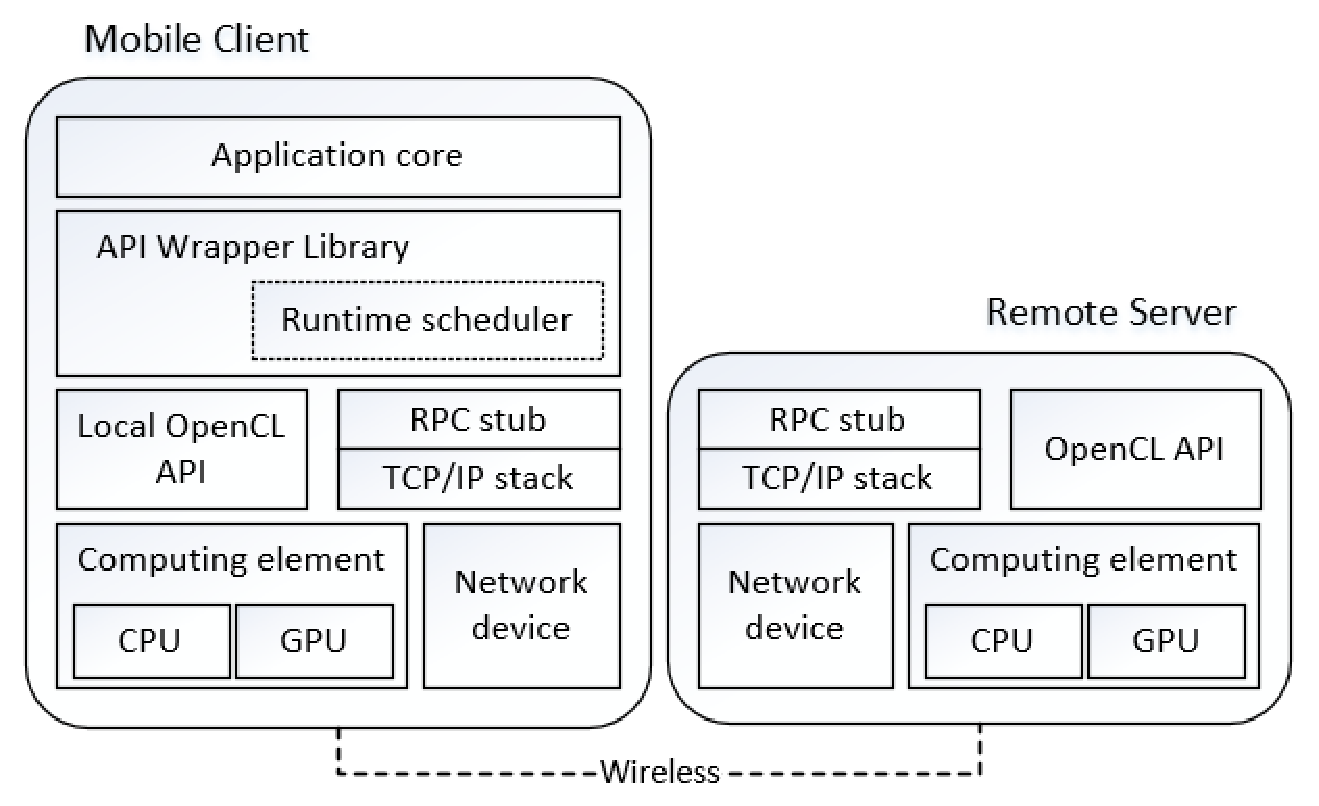
\includegraphics[height=4.5cm, width=8.0cm]{Figure/figure1}
\caption{Overall architecture of the OpenCL-based remote offloading
framework for mobile platforms}
\end{figure}
%
\subsection{Mobile Offloading Framework}
OpenCL is the open standard for parallel programming of heterogeneous
systems, which are increasingly found in personal computers, servers and
mobile devices.
%
By offloading computations to more powerful computing
elements such as Graphics Processing Units (GPUs) or special hardware
accelerators (e.g. SSL accelerators or FPGA) at the hardware layer,
it is possible to improve the performance for a wide range of
applications from gaming and entertainment to scientific and medical
software~\cite{opencl}.
%
The offloading mechanism considered in this study leverages the OpenCL
API to support the remote offloading over the network.
%
As such, the framework inherits the ability of heterogeneous computing of 
the OpenCL standard. 
%
The key idea of the OpenCL-based remote offloading framework (Figure 1) is to
integrate the OpenCL API with an RPC-based service through an API wrapper
library which has an identical name and signature as the original OpenCL
API.\\
%
%Figure 1 depicts the overall architecture of the OpenCL-based remote
%offloading framework.\\
%
\indent When an application invokes an OpenCL API, the API wrapper
library captures this API call, and a runtime scheduler makes a decision
on offloading or local execution.
%
If the scheduler decides to offload the call, it marshalls arguments
for the API and invokes an RPC call associated with the API.
%
Finally, a function is executed on the remote server, and the result is
sent back to the mobile client.
%
On the other hand, if the function should be executed locally, the wrapper
library calls the local OpenCL API and the execution result is returned
to the application directly.\\
%
%\indent Although there exist several options to provide the remote
%procedure call service, serialization, and networking tasks such as
%SunRPC or XMLRPC, they also provide many extra features that are not
%necessarily efficient.
%
%For instance, SunRPC initiates a new TCP connection for each function
%call which incurs extra costs.
%
\indent For an RPC service, we have developed a light-weight marshalling and remote
procedure call layer for our offloading framework.
%an RPC-based service which
%exposes the OpenCL API over the network and uses a single TCP connection
%per offloading job.
%
By running our own RPC-based service, we provide a workload offloading
design that is efficient in terms of argument serialization and buffer
management.
%
\begin{table}
\centering
\caption{Average and standard deviation of network latency and bandwidth
for local and wide area networks including Amazon EC2.}
	\begin{tabular}{c|cc|cc|cc}
	\hline\hline
	\ & \multicolumn{2}{c|}{LAN} & \multicolumn{2}{c|}{Campus network} &
\multicolumn{2}{c}{Amazon EC2} \\
	\hline\hline
	Latency & Avg. & Stdev. & Avg. & Stdev. & Avg. & Stdev.\\
	(\textit{ms}) & 10.833 & 2.684 & 15.465 & 4.189 & 74.036 & 17.737 \\
	\hline 
	Bandwidth & Avg. & Stdev. & Avg. & Stdev. & Avg. & Stdev. \\
    (\textit{MB}) & 6.523 & 0.177 & 2.461 & 0.238 & 0.178 & 0.023 \\ \hline
	\end{tabular}
\end{table}
%
\subsection{Offloading Performance}
In this subsection, we demonstrate the need for support from
adaptive runtime schedulers by conducting an experiment in which we
deploy our offloading framework subject to various network
configurations and collect measurements to show the performance
disparity between different network configurations.\\
%
\indent In the experiments, we utilized an Android tabletPC equipped with
1GHz dual-core processor and 1GB RAM as a mobile client.
%
In order to observe the impact of different network
conditions on the offloading performance, we deployed a remote server
equipped with GeForce GT 640 graphics card into three different network
configurations: local area network, campus network, and Amazon EC2
instance.
%
In the local area network, we connected the mobile client and the remote
server through a wireless router supporting 802.11 b/g/n network
standard.
%
The campus network is used to represent a wide area network in which
the mobile client and the remote server are involved in different
networks: the mobile client connects to the campus wireless router and
the server connects to the laboratory internal router.
%
They communicate each other through multiple routers in the campus.
%
We used an Amazon EC2 GPU cluster as another option for the remote
server located in a wide area network, but for more restricted network
condition than the campus network.
%
Table I summarizes the average and standard deviation of latency
and bandwidth of the network configurations that we setup for the
experiments.\\
%
%\begin{figure}
%	\centering
%	\begin{tabular}{c}
%		\subfloat[Performance for Sobelfilter with different network
%configurations]{\label{fig:figure2-a}
%			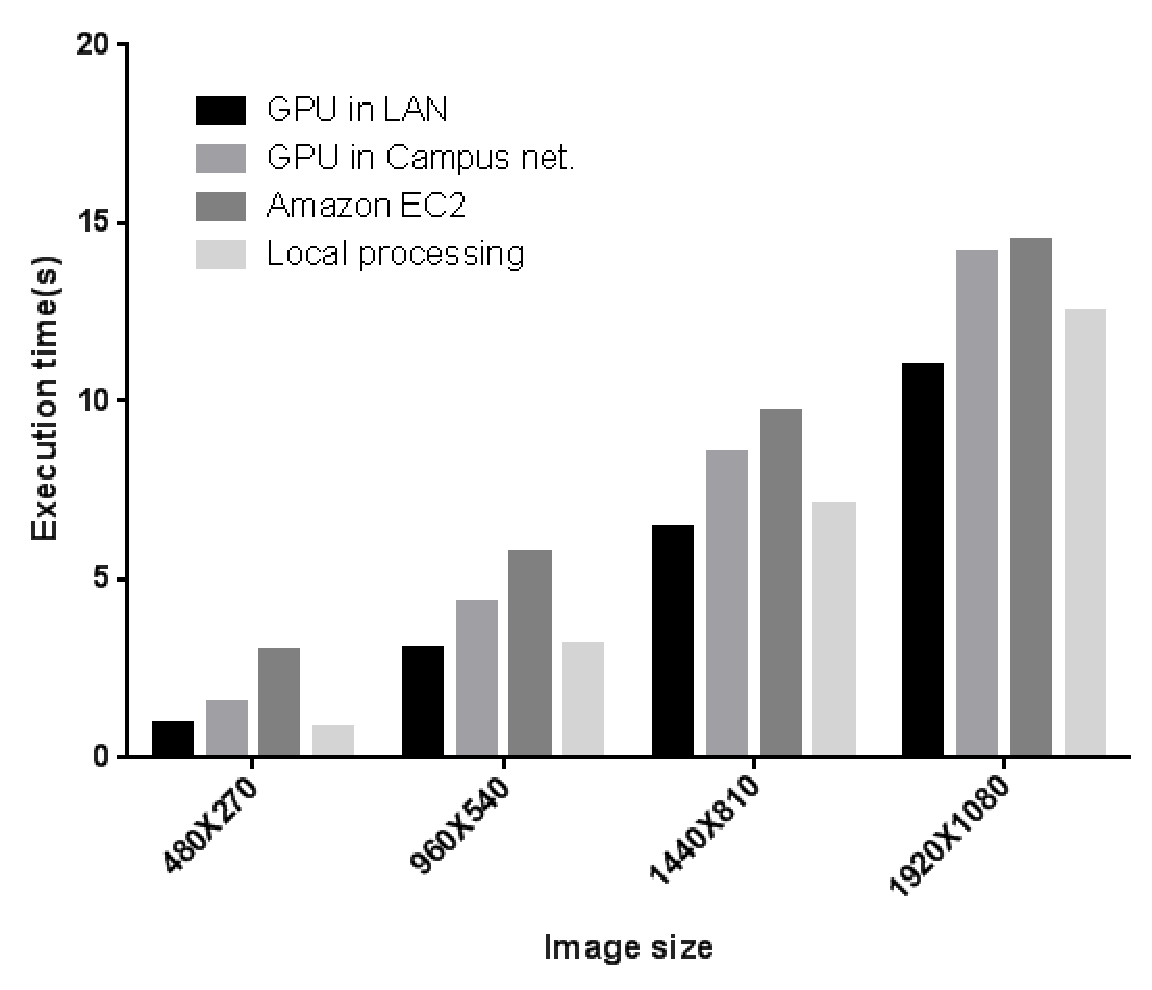
\includegraphics[height=5.6cm,width=7.0cm]{Figure/figure2-a.eps}}\\ 
%		\subfloat[Performance differences between different
%workloads]{\label{fig:figure2-b}
%			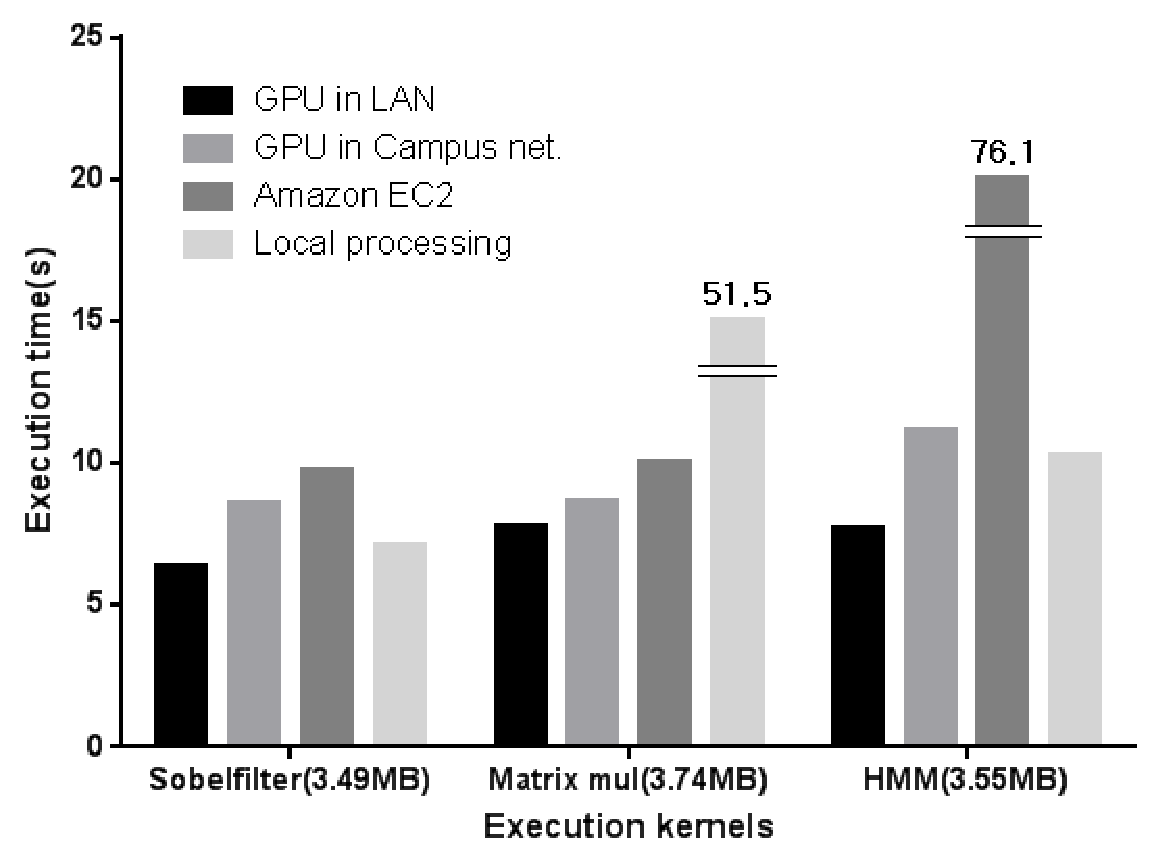
\includegraphics[height=5.4cm,width=7.0cm]{Figure/figure2-b.eps}}\\
%	\end{tabular}
%	\caption{Comparison of total execution time for four OpenCL
%workloads with various servers and network setup}
%\end{figure}
%
\begin{figure}
 	\centering
		\subfigure[Performance for Sobelfilter with different network
configurations]{
			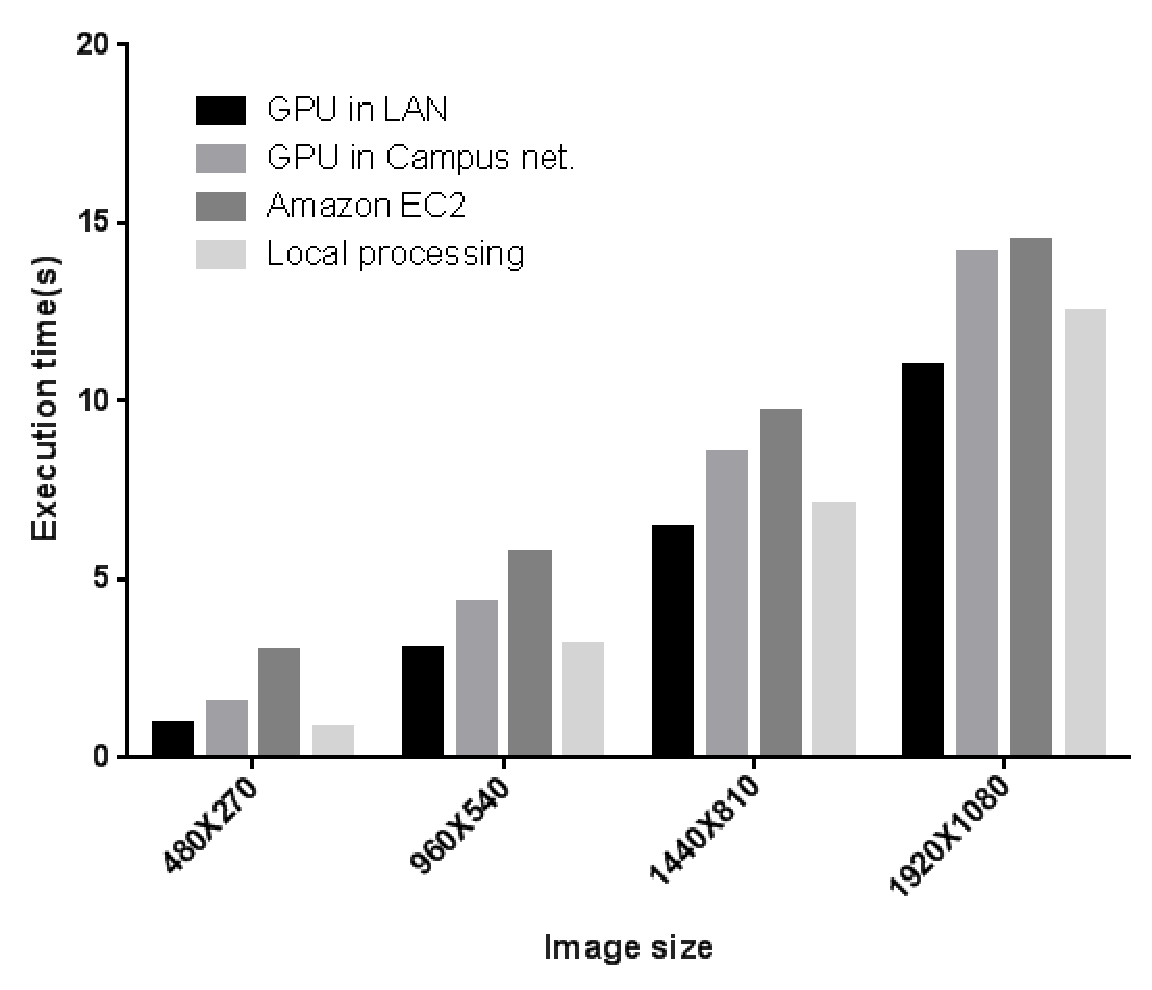
\includegraphics[height=5.6cm,width=7.0cm]{Figure/figure2-a}}\\ 
		\subfigure[Performance differences between different
workloads]{
			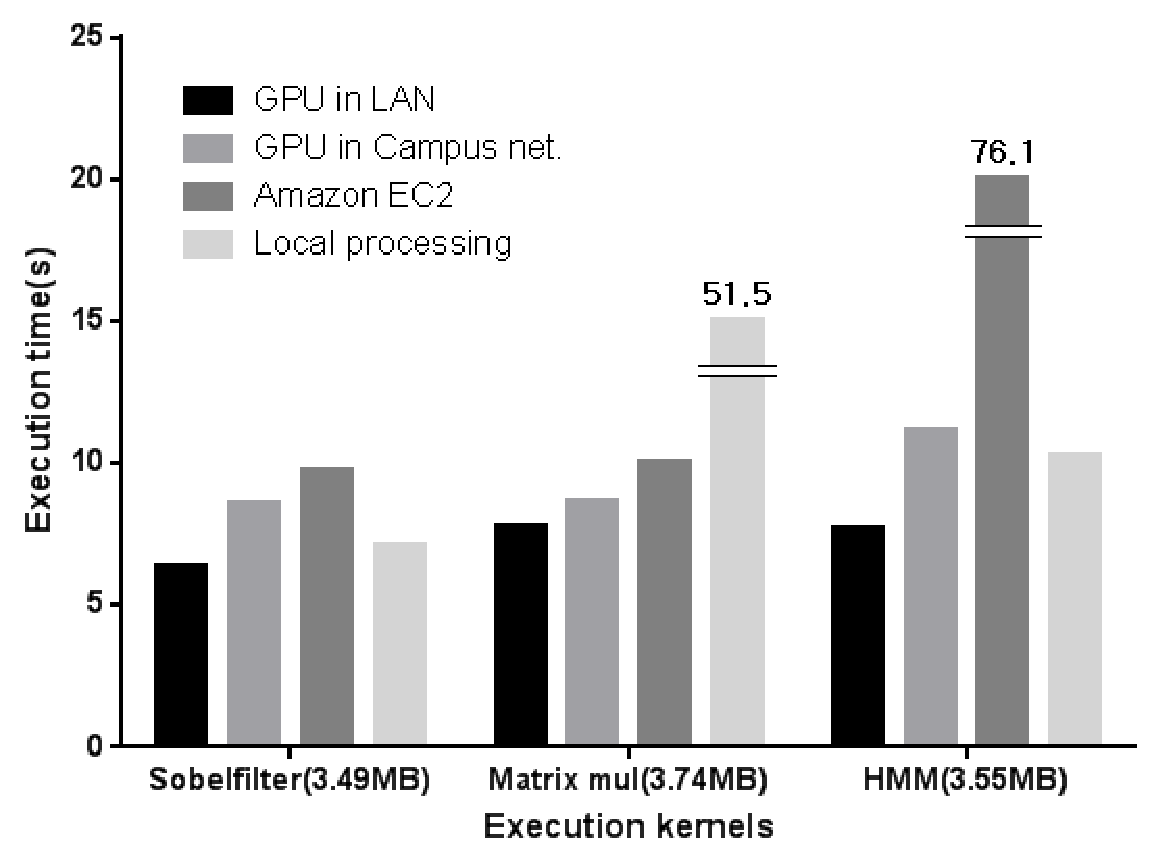
\includegraphics[height=5.4cm,width=7.0cm]{Figure/figure2-b}}\\
	\caption{Comparison of total execution time for four OpenCL
workloads with various servers and network setup}
\end{figure}
%
\indent The benchmarks used in the experiment are Sobelfilter, floating-point
matrix multiplication, Hidden Markov Model, and \textit{N}-body physics
provided by AMD APP SDK~\cite{amd} and Nvidia~\cite{nvidia} sample code.
%
These execution kernels are used by a variety of applications in areas such as image
processing, physics simulation, and mathematical modeling.\\
%
%Also, we utilized several OpenCL execution kernels provided by AMD APP
%SDK~\cite{amd} and Nvidia~\cite{nvidia} for offloaded workloads such as
%Sobelfilter, floating point matrix multiplication, hidden Markov model, and
%\textit{N}-body physics which are used by a variety of areas such as
%image processing, physics simulation, and mathematical modeling.\\
%
\indent Figure 2 shows the offloading performance in terms of the
execution time compared to the case of local processing according to
the data size and network configurations for four OpenCL execution
kernels.
%
As shown in Figure 2(a), for Sobelfilter, we observed that different
network conditions result in significantly different offloading
performance.
%
Particularly, offloading to the remote server located in a local area
network has better performance than local processing.
%
In contrast, offloading to the remote servers located in the campus network
and Amazon EC2 instance, where we have more restricted network conditions
than a local area network, takes longer time than local processing. 
%
Figure 2(b) shows the performance difference among various execution
workloads due to different computational requirements of workloads 
even though they process or offload the similar size of data ranging 
from 3.49MB to 3.74MB.
%
For Sobelfilter, offloading to the GPU server located in LAN is only
more beneficial than local processing.
%
On the other hand, offloading floating-point matrix multiplication has
always better performance than local processing in our setup due to
heavier computational requirement of floating-point matrix
multiplication.
%
%While only offloading Sobelfilter (algorithm complexity for
%Sobelfilter is \textit{0}($n^{2}$)) to the remote GPU server is more
%beneficial than local processing, offloading has always better
%performance than local processing for floating-point matrix
%multiplication (algorithm complexity for floating-point matrix
%multiplication is \textit{0}($n^{3}$)).
%
In fact, the computation complexity for floating-point matrix
multiplication is \textit{O}($n^{3}$) while that for Sobelfilter is
\textit{O}($n^{2}$).\\
%
\indent It is also worth noting that, for Hidden Markov Model, offloading to 
Amazon EC2 instance shows the worst performance among other cases.
%
This is because that Hidden Markov Model requires extra communications
between the mobile client and the remote server to setup additional
arguments for workload execution.
%
Packets are exchanged at higher latencies in the Amazon EC2 setup
compared with a local area network, which causes performance degradation
since our offloading framework requires that each RPC call is acknowledged 
with a response from the remote server.
%
Consequently, offloading to Amazon EC2 GPU instance, which has the
highest latency among our experimental setups, takes the longest time.
%
These results show that there is variation in offloading performance
between different network conditions and execution workloads.
%
Accordingly, proper scheduling can have a significant impact on the
offloading performance, and remote offloading framework requires the
support from the runtime scheduler.
%
\begin{figure}
\centering
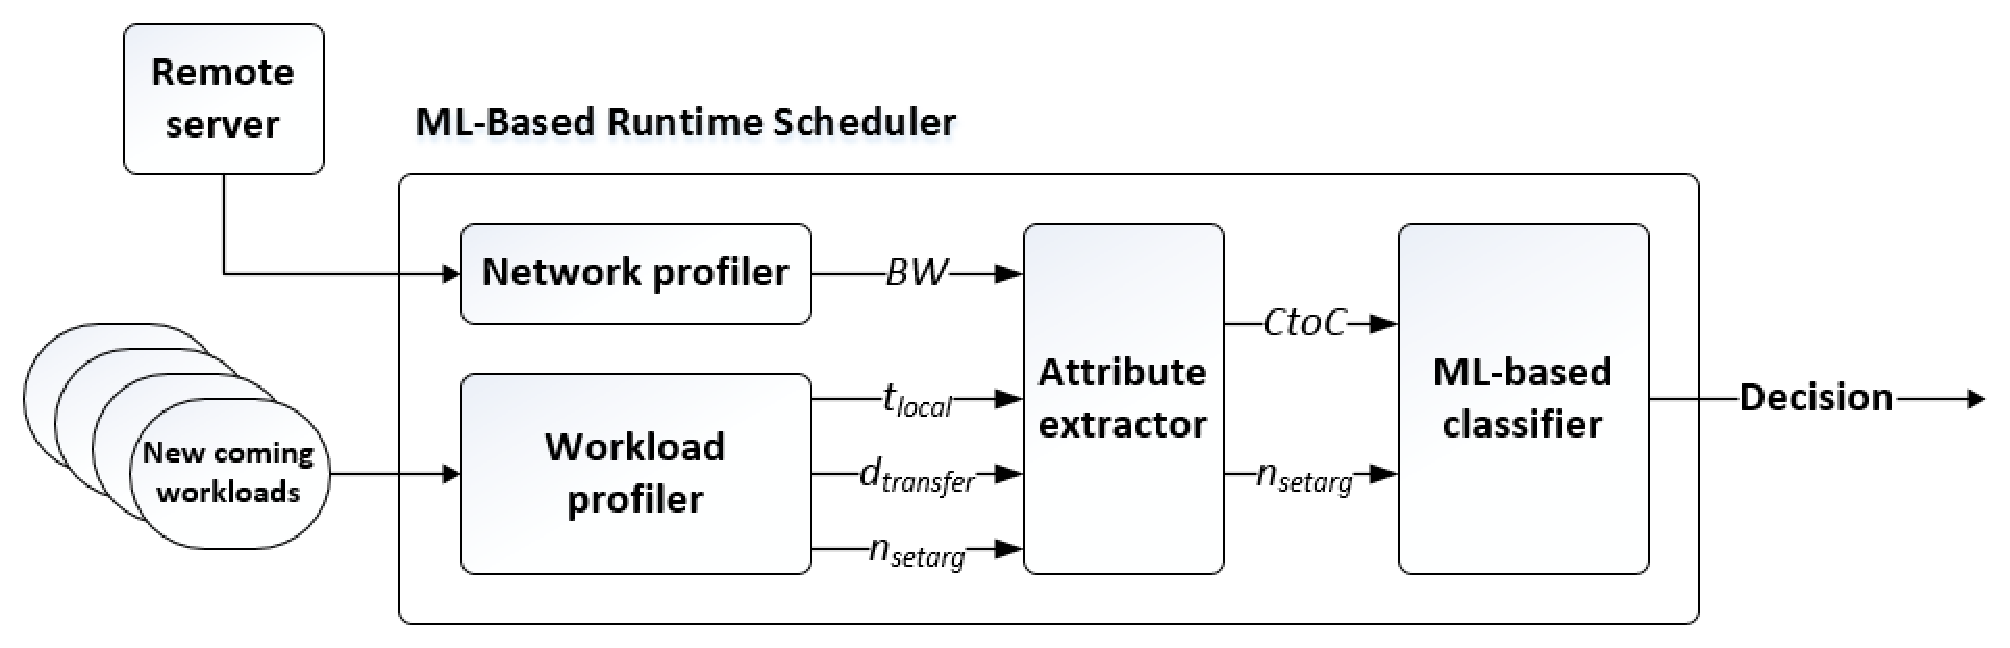
\includegraphics[height=2.8cm, width=8.6cm]{Figure/figure3}
\caption{The structure of Machine Learning-based runtime scheduler}
\end{figure}
%
\section{Machine learning-based runtime scheduler for mobile offloading
framework}
In order to apply machine learning techniques to any decision-making
problems, it is first required to select a subset of relevant
attributes.
%
These need to comprehensively represent a set of problem instances 
in terms of internal and external conditions which have an effect on making a
decision.
%
In this section, we describe the attributes of machine learning
techniques considered in this paper, and how the proposed scheduler can
extract these attributes.
%
Then, using this subset of attributes, we investigate the scheduling
accuracy of machine learning techniques using a dataset collected from
experimental data using benchmark executions.
%
%we investigate the scheduling accuracy of machine lear
%used for the offloading scheduler and how the scheduler
%extracts the attributes from offloading scheduling problems. 
%
%Additionally, using the subset of attributes that we defined for our
%scheduling problem, we investigate the scheduling accuracy of machine
%learning techniques by running an open source machine learning 
%software, Weka, in which various machine learning algorithms are 
%implemented.
%
By taking the text-based dataset as an input, we can train
the classifier of various machine learning algorithms and examine the
accuracy of the trained classifiers.
%
Figure 3 illustrates the structure of our machine learning-based runtime
scheduler and how it generates and uses the subset of attributes to make
a decision for remote offloading framework.
%
%\begin{figure}
%\centering
%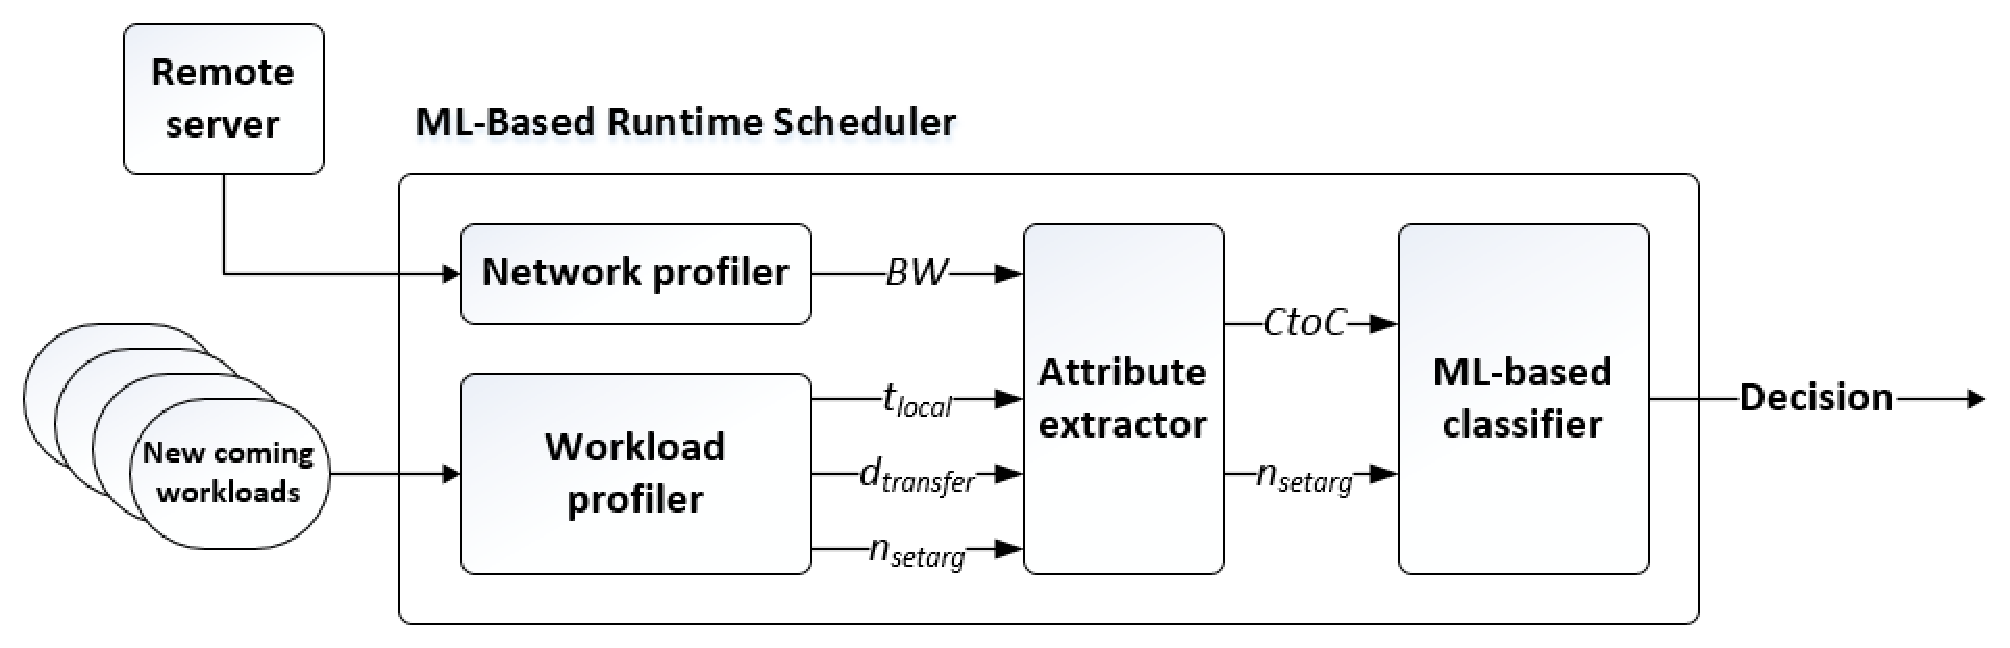
\includegraphics[height=2.5cm, width=8.5cm]{Figure/figure3}
%\caption{The structure of Machine Learning-based runtime scheduler}
%\end{figure}
%
\subsection{Selection of Machine Learning Attributes}
Since offloading performance can vary as a function of network
conditions, the size of data to be processed, and computational
requirements, the scheduler has to take these factors into account to
make an accurate decision on offloading or local processing.
%
We focus on four features to establish the subset of
attributes which is the representation of the scheduling problem for the
remote offloading framework: (1)computation amount of the workload, 
(2)size of data, (3)network bandwidth, and (4)additional communication 
between the mobile client and the remote server to setup extra arguments.\\
%
\textbf{Local execution time(\textit{t$_{local\_execution}$}):} 
We regard the time for a workload to be executed in the mobile client 
locally as the computation amount. 
%
There are a variety of methods to measure the computation amount of the
execution, such as counting the number of assembly instructions or loop
iterations, some of which require additional assistance from the special
hardware or compiler.
%
Instead, in the proposed approach, runtime measurements are taken by the
offloading framework as it executes the workload with the given data
locally, and the scheduler profiles the execution time for the
workload.\\
%
%we utilized an intuitive, yet acceptably efficient way in which
%the framework executes the workload with the given data locally and
%the scheduler profiles the execution time for the workload.\\
%
%TODO: why this is a good method!!
%
\textbf{Size of data to be transferred(\textit{d$_{transfer}$}):}
In addition to the computation cost of a workload depending on the size
of the data, the data size also affects the communication cost to
transfer the data from the mobile client to the remote server.
%
%Even though the computation complexity of workloads already reflects the
%size of data since the local execution time may be varied with the
%given size of data, the data size also affects the communication cost
%to transfer the data from the mobile client to the remote server.
%
In our OpenCL-based remote offloading framework, the APIs for buffer
management such as \textit{clEnqueueWriteBuffer} and
\textit{clEnqueueReadBuffer} are used to profile the size of data to be
transferred.\\
%
\textbf{Network bandwidth(\textit{BW}):} We integrate the network
bandwidth measurement into the offloading framework so that it is able
to measure network bandwidth between the mobile client and the
remote server during runtime.
%
In our implementation, network bandwidth is simply measured by the
size of probing packets divided by the elapsed time to send those
packets~\cite{bandwidth}.\\ 
%
\textbf{Number of the invocations for argument
setup(\textit{n$_{argset}$}):} We count the number of the invocations of
the specific OpenCL API called \textit{clSetkernelArgs}, which causes
additional communication overhead between the client and the server to
setup the extra arguments for kernel executions in addition to the
primary data setup.
%
The reason why we distinguish communications between main data transfer
and additional arguments setup is that, though the latter incurs minor
amount of data, it can cause significant communication costs due to
protocol round-trip messages between the client and the server.\\
%
\indent Note that, rather than considering the local execution time, the
size of data transfer, and network bandwidth as individual attributes
separately, we use \textit{Computation-to-Communication ratio} in which
three features are merged into one attribute as Equation 1. 
%
\begin{equation}
\begin{split}
%\setlength{\arraycolsep}{0.0em}
%\begin{eqnarray}
	CtoC& = t_{local\_execution}\:/\: t_{data\_transfer} \\ 
        & = t_{local\_execution}\:/\:(d_{transfer}\:/\:BW)
%\end{eqnarray}
%\setlength{\arraycolsep}{5pt}
\end{split}
\end{equation}
%
where \textit{t$_{data\_transfer}$} is the time for data transfer.
%
Thus, in our work, computation-to-communication ratio is a composite
measurement which combines three dynamic features into one parameter.
%
As a result, the proposed machine learning-based classifier accepts two
attributes:
computation-to-communication ratio(\textit{CtoC}) and the number of
invocations of \textit{clSetKernelArgs}(\textit{n$_{argset}$}) to make a
decision on scheduling a new workload (i.e. local processing or remote offloading).
%
\begin{figure}
\centering
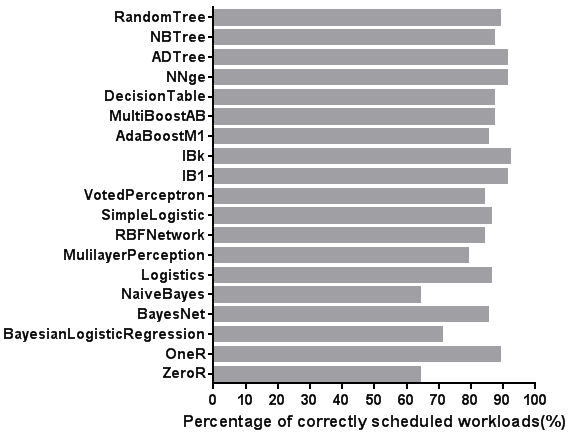
\includegraphics[height=6.0cm, width=8.0cm]{Figure/figure4}
\caption{Offloading scheduling accuracy of various machine learning
algorithms.
% 
The scheduling accuracy from the test dataset(30\% of 640
dataset instances).}
\end{figure}
%
\subsection{Scheduling Accuracy of Machine Learning Techniques}
In this subsection, we investigate the scheduling accuracy of the
machine learning-based scheduler for remote offloading framework.
%
First of all, by running the OpenCL-based offloading framework into
the experimental setup with various network configurations, execution
kernels, and data sizes, we gathered a total of 640 data instances to train 
and test the classifiers of various machine learning algorithms.
%
Each data instance means one execution of the offloading framework, and
consists of \textit{d$_{transfer}$}, \textit{BW}, and
\textit{n$_{argset}$}.
%
Next, we aggregate collected data instances to create the
training and test datasets, each consisting of a 3-tuple, $\{$\textit{CtoC},
\textit{n$_{argset}$} ; \textit{label}$\}$, with two attributes explained 
in the previous section and the label which is a decision on 
\textit{offload} or \textit{local}.
%
Then we labeled each data instance by comparing offloading 
performance to the local execution in terms of the execution time.
%
For example, if offloading Sobelfilter with a 1920$\times$1080 image
into a machine with a GPU in LAN takes a shorter time than
local processing, the instance is labeled as \textit{offload}.
%
In our collected dataset, 65\% of instances are labeled as
\textit{offload}.
%
Note that it is possible to use another performance metric: mobile
device's energy consumption, such that each instance can be labeled
based on energy consumption between remote offloading and local
processing.
%
%To do this, we first gathered total 448 training data instances by
%deploying the OpenCL-based offloading framework into the experimental
%setup with various network configurations(LAN, campus network and Amazon
%EC2) and execution kernels(Sobelfilter, matrix multiplication, hidden
%Markov model and \textit{N}-body physics) as described in Section III.B.
%
%We also vary the size of data for each workload to change the local
%execution time and the data transfer time.
%
%We labeled the collected instances by comparing offloading performance
%to local execution in terms of the execution.
%
%For example, if offloading Sobelfilter with 1920$\times$1080 of image size
%into a GPU machine in LAN takes shorter time than local processing, this
%instance is labeled as \textit{offloading} and vice versa.
%
%Note that it is possible that each instance can be labeled using the
%different performance metrics such as energy consumption or the mobile
%device rather than the execution time.
%
Lastly, we separated the collected dataset with 70\% of them for
the training dataset and the rest for the test dataset, so they have
the identical distribution for instance properties.\\
%
\indent Using the training dataset, 
we trained the classifiers of various categories of machine learning 
algorithms such as Decision Tree, Bayesian Networks, Instance-Based
Learning, and Perceptron-Based Learning.
%
In the training phase, Weka takes the text-based training dataset as
the input and automatically generates the classifier associated with
each machine learning algorithm.
%
Once each classifier is trained, we tested the accuracy of the
trained classifier with the test dataset by observing whether the trained classifier labels each
instance in the test dataset correctly or not.\\
%
\indent Figure 4 shows the scheduling accuracy of various machine learning
algorithms.
%
In this evaluation, the scheduling accuracy is calculated through the
number of the correct decisions made by the classifier out of the test
dataset.
%
We observed that two Instance-Based Learning classifiers performed 
the most accurate prediction, showing greater than 90\% of the scheduling
accuracy.
%
%We observed that Instance-Based Learning classifiers such as
%\textit{1}-Nearest Neighbor and \textit{3}-Nearest Neighbor performed
%the most accurate classifications showing 91.09\% and 92.14\% of the 
%scheduling accuracy while Naive Bayes classifier has the worst
%performance, 64.39\% of the accuracy, among various machine learning 
%algorithms we used to examine the scheduling accuracy. 
%
The basis for the classification of Instance-Based Learning is the instances 
database, where previously seen instances are stored.
%
Instead of building the explicit classifier as other machine learning
algorithms, Instance-Based Learning compares a new problem instance with the stored
instances in the database to select \textit{k} most similar instances 
from the database and votes the majority of the selected instances to 
predict the label of the new problem instance.
%
\textit{k} set to 1 (IB1) and 3 (IB3) as higher values showed the same
performance. 
%
%Since IBL uses all the stored instances in the database for the
%generalization of new problem instances, it does not have any
%information loss from previously seen instances.
%
The classification of probabilistic machine learning
techniques such as Bayesian Networks is based on the statistics
of attributes of the previous instances such as the mean and the
variance values.
%
Thus it is possible that probability-based machine learning
algorithms overlook the edge of previously seen instances, which causes
the performance degradation for the prediction problem. 
%
In fact, Naive Bayes has the worst performance among machine learning
algorithms used for the evaluation, showing 64.4\% scheduling
accuracy.
%
\section{Performance evaluation for offline scheduler}
%
In this section, using the classifiers from various machine learning
algorithms, we implement an offline offloading scheduler and evaluate
the performance and penalty of the offline runtime schedulers.
%
\subsection{Experimental Setup}
Based on scheduling performance and algorithm complexity, we selected
three machine learning algorithms: RandomTree, Instance-Based Learning
and Rule-Based Learning, and built them onto our remote offloading
framework for the offline runtime scheduler.
%
For RandomTree, we used the classifier that Weka generated using the
training dataset described in Section IV.B.
%
Total depth of the tree is 101 and the scheduling accuracy simulated
through Weka is 89.5\%.
%
Though we do not need any classifier for Instance-Based Learning
algorithm, it is required to define the similarity between a new problem
instance and previously stored instances in the database.
%
To do this, we used Euclidean distance, which is common to measure the
similarity for Instance-Based Learning~\cite{instance}.
%
The closer the distance between instances is, the more similar 
they are.
%
We stored the training dataset with 448 instances to build the
database for the Instance-Based Learning algorithm.
%
For simplicity, we use \textit{k=1} for Instance-Based Learning
algorithm.
%
For Rule-Based Learning, we establish a simple rule based on
computation-to-communication ratio threshold, in which the scheduler
decides to offload the mobile computation only if
computation-to-communication ratio is higher than the threshold.
%
Based on our observation, it is most likely that the benefits from
offloading are more promising when computation-to-communication ratio is
higher than 1.5.
%
For that reason, we setup the threshold with 1.5 and 3.\\
%
\indent Also, we emulate various network configurations in which the
client and the server connect directly through a wireless router, but
have 9 different network bandwidths ranging from 6.5MB/s to 0.3MB/s
controlled by Traffic Control (TC)~\cite{tc}.
%
TC is a network tool which provides functionalities to control network
traffic by prioritizing network resources and using concepts of traffic
classification, queue disciplines and quality of service (QoS).
%
While setting different network bandwidths, we ran
our offloading framework with four benchmark kernels 720 times (9
network bandwidths $\times$ 4 kernels $\times$ 4 data sizes $\times$ 5
repeats for average) per each offline scheduler.
%
\subsection{Performance Comparison}
%
Figure 5 shows the scheduling accuracy for various machine learning
algorithms with four benchmark kernels.
%
%We also added two extreme schedulers with the simple scheduling policy,
%all offloading and all local execution for performance comparison.
%
Similarly as the result shown in Figure 4, we observed that
Instance-Based Learning has the most accurate scheduling performance
among various schedulers showing 92\% of the scheduling accuracy.
%
Even though in matrix multiplication and Hidden Markov Model,
other machine learning algorithms have better performance than Instance-
Based Learning,
%Instance-Based Learning due to the appropriateness of each scheduler to
%the characteristics of the certain execution kernel, 
Instance-Based Learning shows the best performance on average.
%
It is also observed that, even though the schedulers based on Rule-Based
Learning algorithm consider only one attribute,
computation-to-communication ratio, they have better performance than
RandomTree.
%
An interpretation is that the computation-to-communication ratio is a
more dominant attribute than the number of argument setup, \textit{n$_{argset}$}.
%
Interestingly, for \textit{N}-body physics, all machine learning
algorithms show the perfect scheduling accuracy.
%
It is because that computation-to-communication ratio for
\textit{N}-body physics is extremely high in our experimental setup
so that it is easy for the scheduler to differentiate the conditions 
where offloading or the local execution for \textit{N}-body physics 
is more beneficial than the other.
%
In fact, offloading \textit{N}-body physics always had better
performance that the local execution in our setup.\\
%
%As a result, all offloading policy has the ideal scheduling accuracy as
%well.\\
%
\begin{figure}
\centering
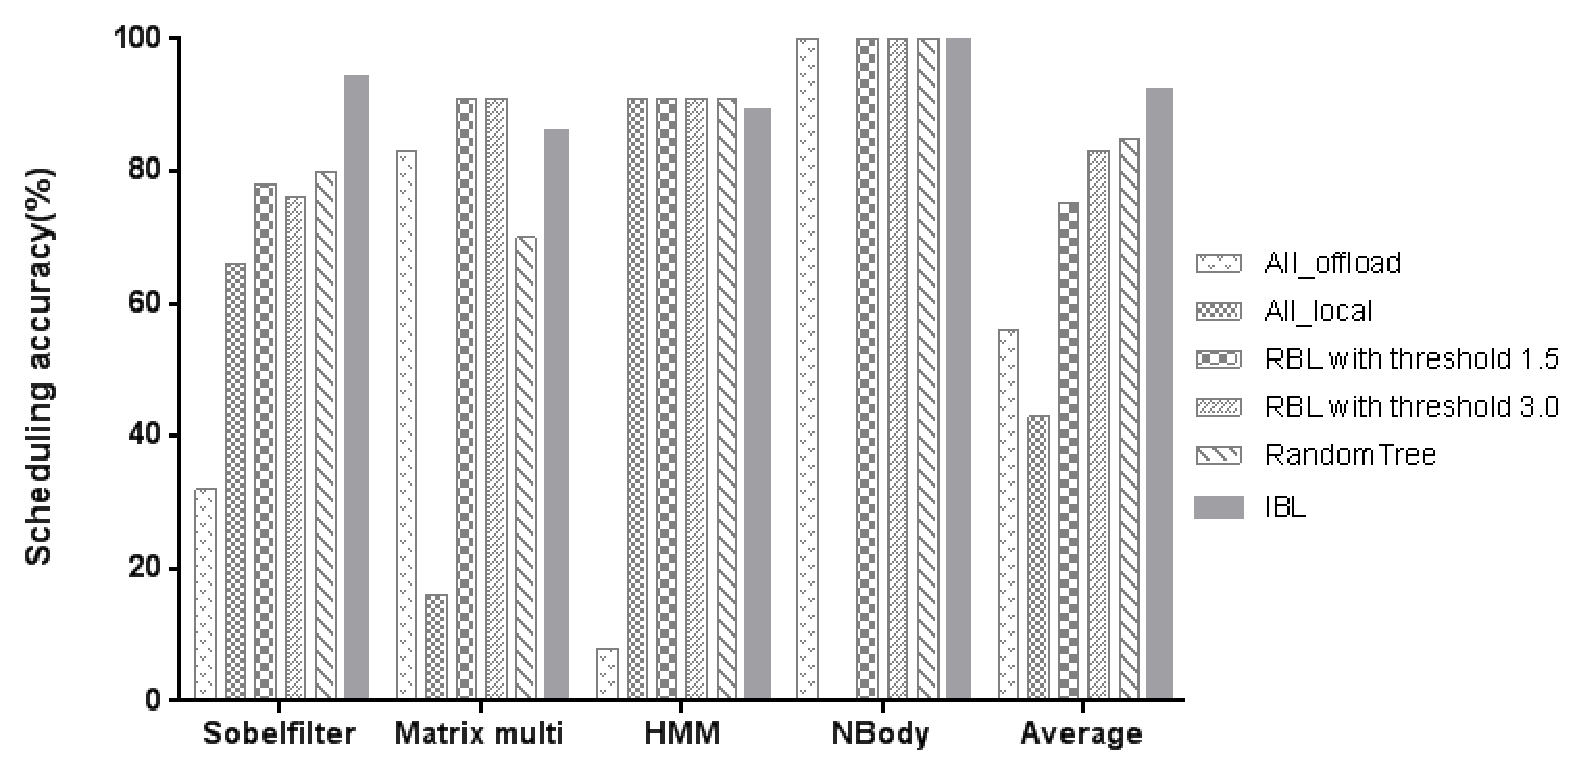
\includegraphics[height=4.3cm, width=8.5cm]{Figure/figure5}
\caption{Scheduling accuracy of the offline schedulers using various
machine learning algorithms.
%
For performance comparison, we also added two simple scheduling policies,
all\_offload and all\_local which are not machine learning algorithms.}
\end{figure}
%
\indent Figure 6(a) and (b) present the penalty for various schedulers
normalized to the case of the oracle scheduler which always makes the
right decision to offload or run locally as Equation 2.
%
%various schedulers 
%normalized to the case of the oracle scheduler which always makes the
%right decision to offload or run locally.
%
%\setlength{\arraycolsep}{0.0em}
%\begin{eqnarray}
\begin{multline}
	penalty_{normalized} \\ 
			= (execution\_time_{ML} 
              - execution\_time_{oracle}) \\
                 / execution\_time_{oracle}
\end{multline}
%\end{eqnarray}
%\setlength{\arraycolsep}{5pt}
%
where \textit{execution\_time$_{ML}$} and 
\textit{execution\_time$_{oracle}$} are the processing times 
of the workload scheduled by the machine learning-based scheduler 
and the oracle scheduler, respectively.
%
For the penalty in terms of energy consumption, 
\textit{execution\_time$_{ML}$} and \textit{execution\_time$_{oracle}$}
should be replaced with the mobile device's energy consumption to 
execute or offload the workload scheduled by each scheduler.
%
In our evaluation, the penalty implies the extra costs that the mobile
device or user has to pay additionally over the oracle scheduler when
the machine learning-based scheduler makes a wrong decision. 
%
To profile energy consumption of the mobile device, we used
PowerTutor~\cite{powertutor} which is an application for the variants of
Android devices that displays the power consumed by major components
such as CPU, network interface, LCD display, and GPS receiver.\\
%
\indent As you can see, the Instance-Based Learning scheduler has the smallest
penalty in terms of the execution time because it has the highest
scheduling accuracy.
%
For energy consumption, moreover, the Instance-Based Learning scheduler has
a fairly small penalty compared with Rule-Based Learning scheduler.
%  
Note that, for Sobelfilter, the penalty in terms of both the execution
time and energy consumption is lower than other execution kernels,
because the gap of the execution time and energy consumption for
Sobelfilter between offloading and the local execution is relatively
small.
%Note that, for \textit{N}-body physics, the penalty in terms of both the
%execution time and energy consumption is higher than other execution
%kernels, because the execution time and energy consumption for
%\textit{N}-body physics are very big compared with those for offloading.
%the gap of the execution time and energy consumption
%for \textit{N}-body physics between offloading and the local execution
%is very big.
%
Therefore, the penalty for Sobelfilter is less significant than the
cases of other execution kernels when the scheduler makes a wrong
decision on offloading or the local execution.
%
\begin{figure}
	\centering
		\subfigure[Execution time]{
			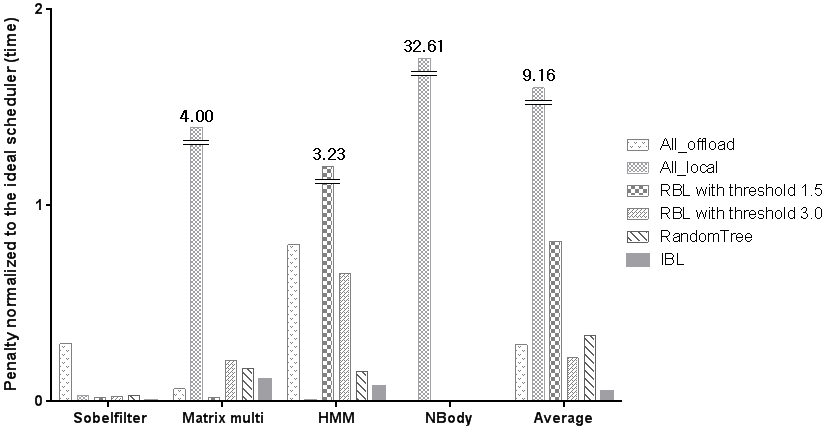
\includegraphics[height=4.8cm,width=8.5cm]{Figure/figure6_1}}\\ 
		\subfigure[Energy consumption]{
			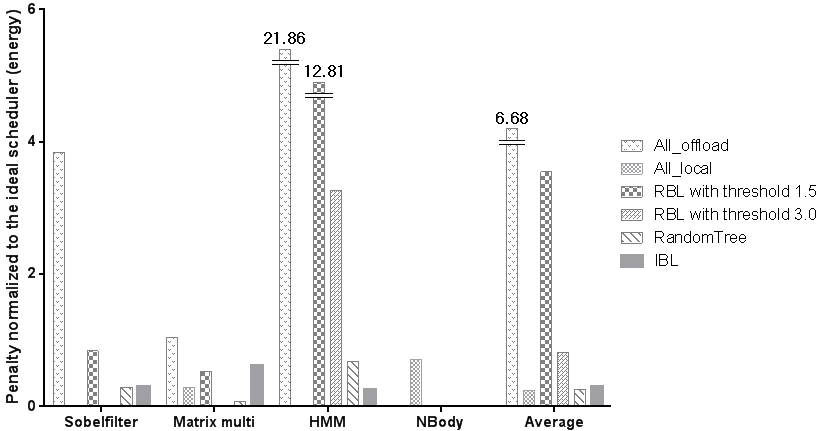
\includegraphics[height=5.0cm,width=8.5cm]{Figure/figure6_2}}\\
	\caption{Penalty normalized to the oracle scheduler in terms of
the execution time and energy consumption}
\end{figure}
%
\section{Online runtime scheduler}
In the previous section, we demonstrated the offline runtime offloading
scheduler based on various machine learning algorithms by illustrating
the scheduling accuracy and the penalty with regard to the execution
time and energy consumption of the mobile platforms.
%
In this section, we explore the potential possibility and benefits of an
online runtime scheduler for mobile offloading framework in which
the online scheduler can be trained through the previous experiences
automatically and adapt to the dynamic situation.
%
%We implement the online offloading scheduler based on
%Instance-Based Learning algorithm and evaluate it from a perspective of
%the adaptiveness of the dynamic change of network conditions.
%
\begin{figure}
\centering
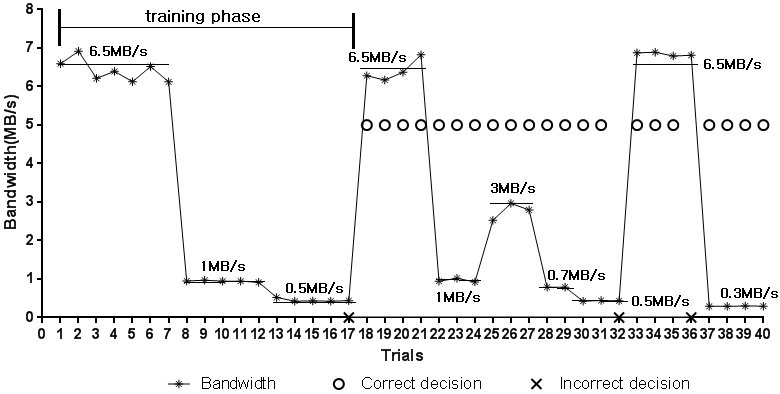
\includegraphics[height=4.8cm, width=8.5cm]{Figure/figure7}
\caption{The ability to adapt dynamic network conditions for the online
offloading scheduler}
\end{figure}
%
\subsection{Implementation of the Online Offloading Scheduler}
We first implemented the prototype of the online runtime scheduler
based on the Instance-Based Learning algorithm for the mobile offloading
framework.
%
The reason why we chose the Instance-Based Learning algorithm for the
online runtime scheduler is due to the simplicity of the algorithm and
the ability to quickly apply newly seen data to its future decisions.
%
Usually, other machine learning algorithms such as neural networks or
linear regression have its own the classification model and it is
required to be completely modified when a new instance data is added to
the training dataset.
%
%Instead of requiring the classification model to be completely modified
%when a new instance data is added to the training dataset,
%Instance-Based Learning simply stores the new instance to the training
%dataset, and the new instance is used to predict a next coming problem
%instance along with previous stored instances.
%
However, Instance-Based Learning simply stores the new instance to the
training dataset, and the new instance is used to predict a next coming
problem instance along with previous stored instances.
%
In addition to its simplicity, in our evaluation for the offline offloading scheduler,
Instance-Based Learning showed the best performance among various
machine learning algorithms we used for the evaluation.\\
%
\indent The following is the scheduling process of our prototype of the online
scheduler.
%
Once the application starts, the online scheduler executes the
application locally at once to figure out the information which is
required for profiling the workload such as the local execution time, the
size of data, or the number of the invocations for argument setup.
%
Then, the scheduler enters the training phase by unconditionally
offloading the execution to the remote server \textit{N} times, and
each case is labeled according to the performance comparison between
offloading and the local execution.
%
The labeled instance is stored into the training database.
%
For our prototype, we set \textit{N} with 16.
%
After the training phase, the scheduler starts the scheduling process by
measuring the Euclidean distance between a new scheduling problem and
the instances stored in the training database.
%
When offloading is scheduled, the scheduler offloads the workload and 
measures the execution time for offloading.
%
If offloading takes shorter than the local execution, then that instance
is added to the training database as \textit{offload}.
%
On the other hand, it is stored as \textit{local}.\\
%
%It is worth noting that there is the difference on the update process of
%the training database between when offloading and the local execution
%are scheduled.
%
\indent To update the training database, the scheduler keeps adding the
new instance to the database without removing any previous stored
instance until the database is full.
%
Only if the database is full, the oldest instance will be replaced with
the new one.
%
For our implementation, we try to find the optimal number of instances for
the database which covers as many cases as possible, but takes reasonably small 
memory space (less than 1MB) and time (less than 0.01sec) to schedule a
new problem.
%
We chose 5,000 instances database which requires only 0.1MB of memory.
%
This memory usage occupies only less than 0.0007\% of typical memory
sizes of
contemporary mobile devices (e.g 16GB or 32GB).
%
Also, even though it takes 5$\sim$6msec to measure the Euclidean
distance of the new scheduling problem with 5,000
instances, we believe that instance generalization or clustering techniques for
the database such as~\cite{domingos, chang} can help the
scheduler significantly reduce the measurement time. 
%
\subsection{Evaluation for the Online Scheduler}
In order to evaluate the prototype of our online scheduler, we conducted
an experiment in which we change network conditions and observe how
well the scheduler learns and adapts to dynamic network conditions.
%
In this experiment, the client and the remote server are directly
connected through a wireless router and we controlled the network
bandwidth between them using TC.
%
Also, we used Sobelfilter for the offloaded execution kernel.
%
Figure 7 shows the ability to adapt the online scheduler to dynamic
network conditions.\\
%
\indent During the training phase, we setup different network conditions where
the scheduler is trained with three network bandwidths: 6.5MB/s, 1MB/s,
and 0.5MB/s.
%
After the training phase, the scheduler makes a decision on offloading
or the local execution in six different network bandwidths as shown in
Figure 7.
%6.5MB/s,
%3MB/s, 1MB/s, 0.7MB/s, 0.5MB/s, and 0.3MB/s for 40 trials.
%
As you can observe, the scheduler makes the correct decisions in dynamic
network conditions except for 17th, 32nd, and 36th trial.
%
These incorrect decisions are because network bandwidth is changed
after the scheduler makes a decision.
%
As a result, the actual cost for data transfer is different with what
the scheduler predicts. 
%
Furthermore, even at the unseen conditions in the training phase such as
3MB/s or 0.3MB/s, the scheduler works correctly by making right
decisions.
%
Consequently, we observed the possibility and the potential benefits of
machine learning-based online offloading scheduler in this experiment. 
% 
\section{Conclusion and Future work}
In this paper, we proposed machine learning-based runtime scheduler for
mobile offloading framework.
%
Before addressing the scheduling problem of the mobile offloading
framework, we showed the performance variance between different network
conditions and workload characteristics by deploying the OpenCL-based
offloading framework into a local and wide area network.   
%
By running various machine learning algorithms, we also showed the
feasibility of adopting machine learning techniques into the scheduler
problem for mobile offloading framework.
%
In addition, we implemented an offline offloading scheduler
using the classifiers of RandomTree, Instance-Based Learning, 
and Rule-Based Learning.
%
In the evaluation, the scheduler based on Instance-Based Learning
performed 7\% better than RandomTree and 3\% better than Rule-Based
Learning.
%
Finally, using Instance-Based Learning, we demonstrated the potential 
benefits and the ability of the online offloading scheduler to adapt
into dynamic network conditions.\\
%
\indent As the future work, we can extend the online offloading
scheduler by considering the scenario where multiple remote servers are
available.
%
By integrating the functionality to enumerate computing capabilities and
network conditions for multiple servers, the scheduler can make a decision
on not only offloading or the local execution, but also which remote
server is the best to offload the mobile executions.
% 
\section*{Acknowledgment}
This material is based upon work supported in part by the National Science
Foundation under Grant No. 0910812, 0758596, 0855031, and 1265341.
%
Any opinions, findings, and conclusions or recommendations expressed in
this material are those of the author(s) and do not necessarily reflect
the views of the National Science Foundation.
%
\bibliography{ucc13_final}

%\begin{thebibliography}{1}

%\bibitem{IEEEhowto:kopka}
%H.~Kopka and P.~W. Daly, \emph{A Guide to \LaTeX}, 3rd~ed.\hskip 1em plus
%  0.5em minus 0.4em\relax Harlow, England: Addison-Wesley, 1999.

%\end{thebibliography}

% that's all folks
\end{document}


